\chapter{Síťová komunikace a databáze} \label{chap:methods}
Smyslem zkonstruovaných čidel je jejich snadná implementace do bytu či domu. Senzory potřebují kabelově připojit jen napájení a celá komunikace mezi mikročipem a brokerem probíhá po WiFi. Tato schopnost bezdrátové komunikace zásadně rozšiřuje možnosti rozmístění senzorů po domácnosti. Komunikace senzorů se serverem využívá principů \textit{IoT} a síťový protokol \textit{MQTT}. 

\section*{Síť IoT} \label{sec:iot}
Síť IoT\footnote{\textbf{I}nternet \textbf{o}f \textbf{T}hings - internet věcí} je architektura na bázi internetu, která obecně slouží ke komunikaci a výměně dat. Senzory v projektu chytré domácnosti spadají do komponent v internetu věcí, protože veškerá komunikace probíhá po internetu a výhradně bez účasti uživatele. Technologie pro chytrou domácnost v tomto projektu byla navržena tak, aby uživatel měl přísun aktuálních dat ze senzorů bez nutnosti znalosti principů fungování celého systému.

\section{Protokol MQTT} \label{sec:protocol_mqtt}
MQTT\footnote{\textbf{MQ} \textbf{T}elemetry \textbf{T}ransport} je internetový protokol, který slouží k výměně zpráv mezi subjekty v síti. Tento protokol vznikl už v roce 1999, ale k významnému využití dochází i v dnešní době právě díky IoT aplikacím. MQTT pracuje na TCP/IP vrstvě a hodí se především v aplikacích, které vyžadují co nejmenší datový přenos po síti.  \par
Při komunikaci prostřednictvím MQTT protokolu jsou v síti definovány dva typy entit. V síti se nachází server - \textit{broker} a libovolné množství klientů. Veškerá komunikace probíhá prostřednictvím brokeru. Broker je centrální místo v síti, na které ostatní zařízení publikují zprávy a který ostatním subjektům v síti umožňuje číst tyto zprávy. Klientem může být jakékoliv zařízení, které má přístup na internet a podporu MQTT protokolu. Zpravidla jde o chytré senzory, které publikují zprávy. V tomto projektu broker představuje počítač Raspberry Pi (více v \cref{sec:raspberry_pi}) a klienti jsou jednotlivé senzory - mikročipy ESP8266. Princip protokolu MQTT je zobrazen na \cref{fig:mqtt_communication}. Jednotlivé senzory publikují zprávy na broker (mód \textit{publish}) a broker přijímá všechny příchozí zprávy. Další aplikace jako je webový a databázový server odebírají příchozí zprávy (mód \textit{subscribe}) od brokeru za účelem dalšího zpracování dat. Z hlediska protokolu může být jeden klient současně \textit{publisher} i \textit{subscriber}, ale často bývají tyto role rozděleny. \textit{Publisher} je zpravidla chytrý senzor, který měří nějakou fyzikální veličinu a hodnoty odesílá na broker a \textit{subscriber} je většinou zařízení, které čte data zaslaná od \textit{publishera} a s těmito daty pak dále pracuje (například je zobrazuje ve webovém rozhraní nebo ukládá do databáze).  

\begin{figure}[H]
  \centering
  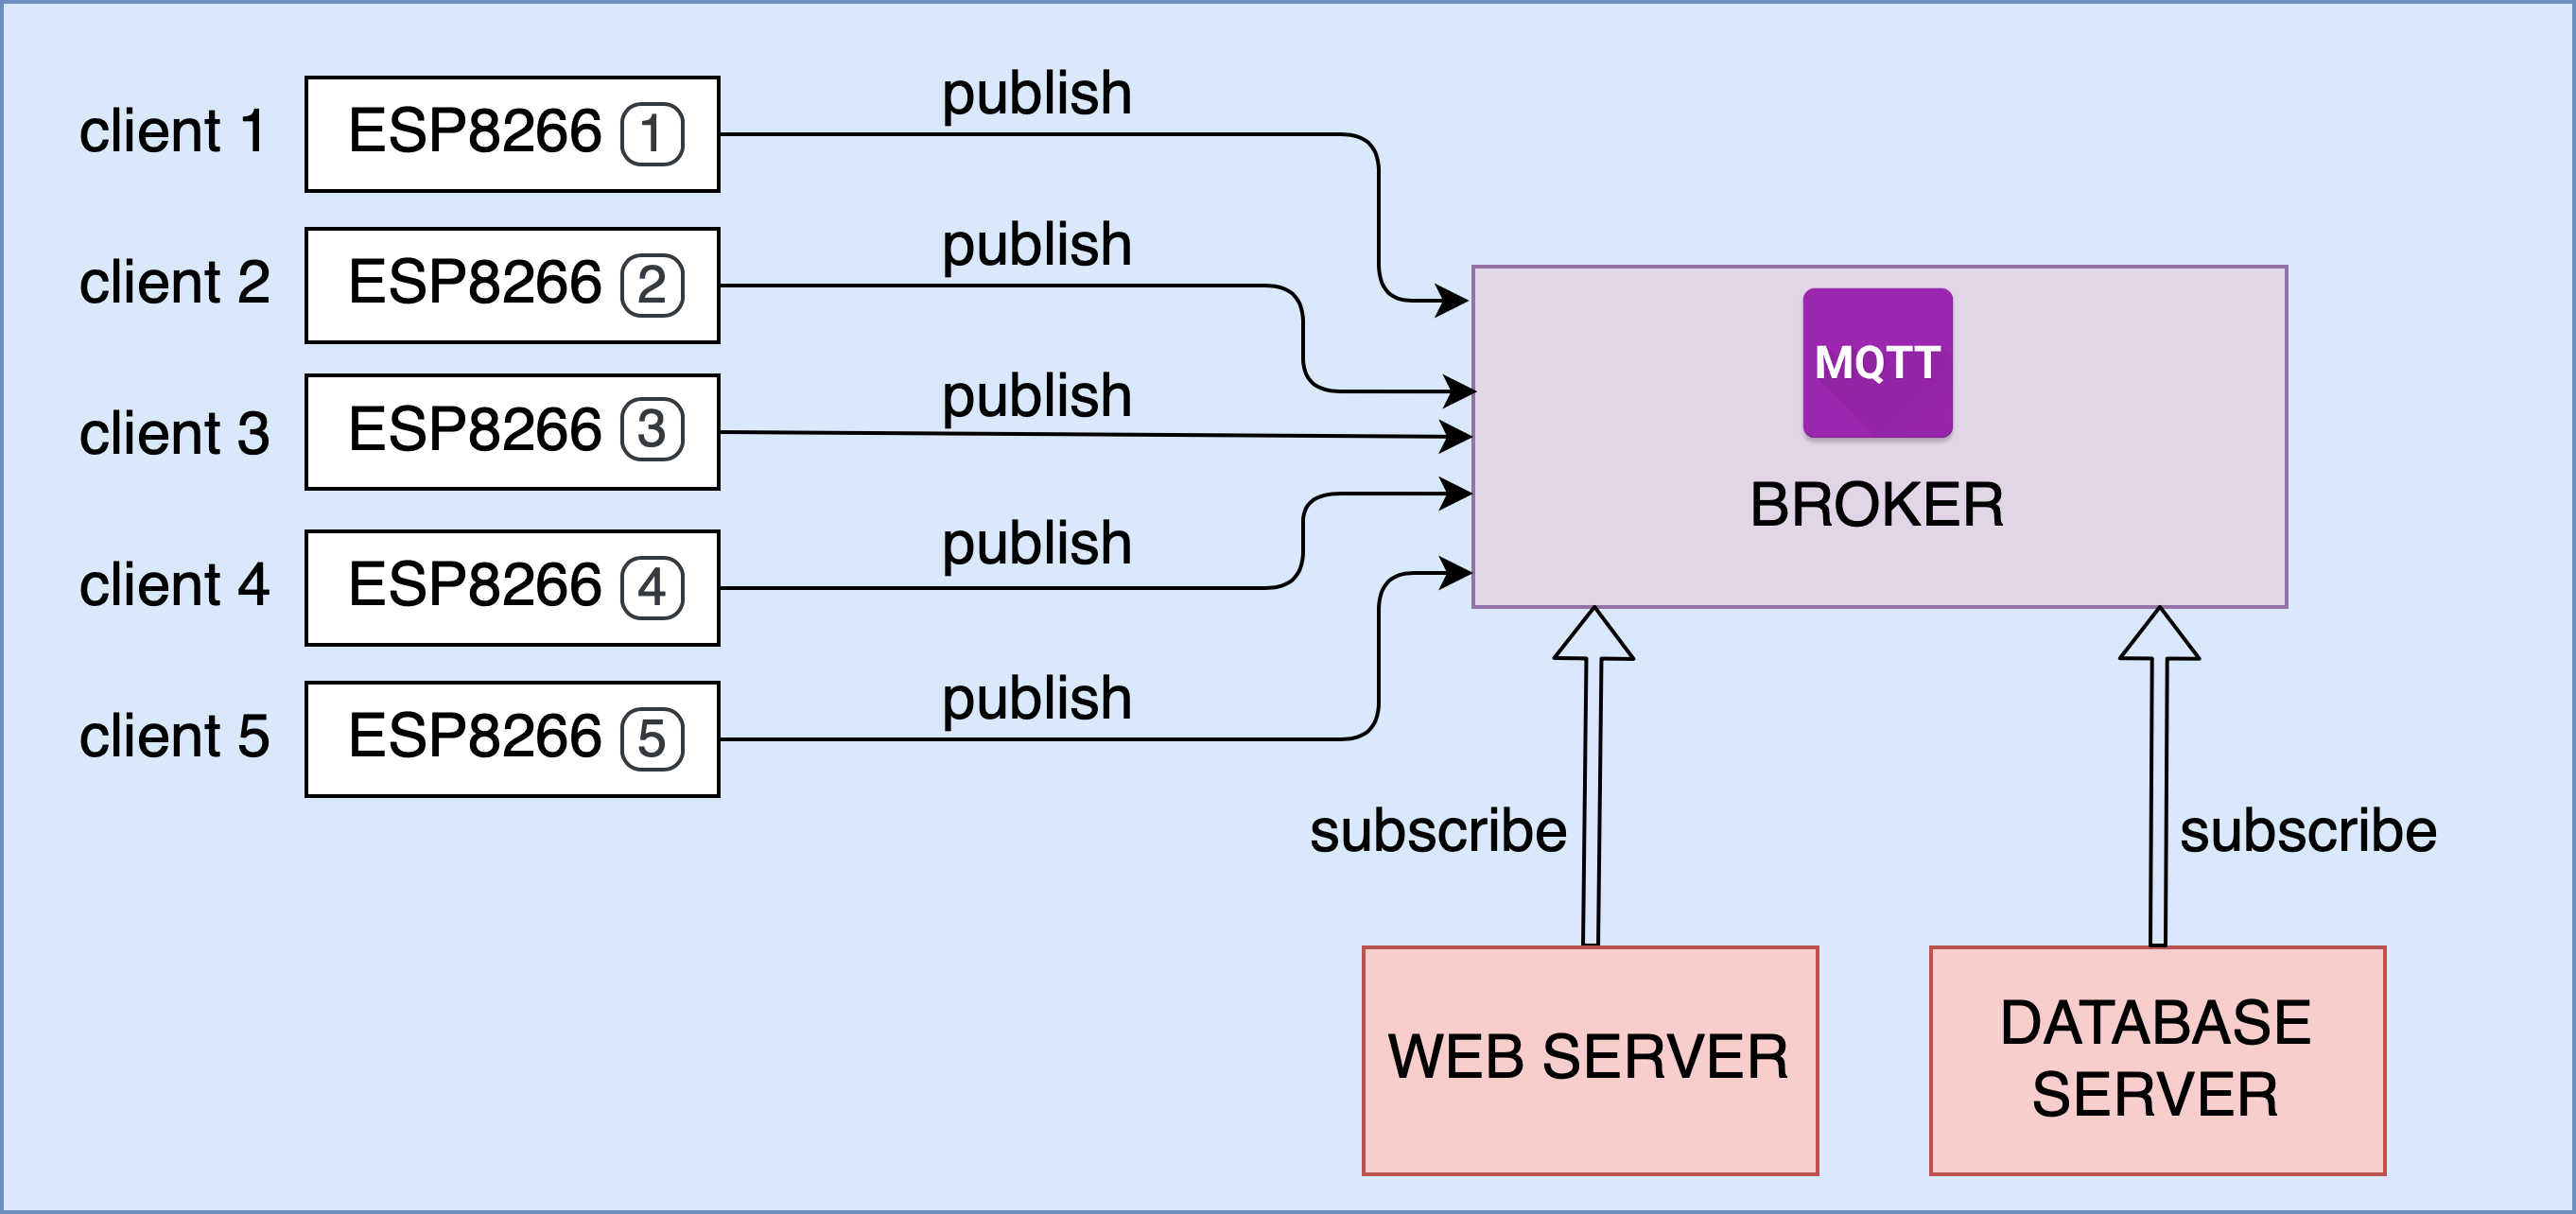
\includegraphics[width=0.7 \textwidth]{mqtt_diagram.png}
  \caption{Princip komunikace přes MQTT protokol}
  \label{fig:mqtt_communication}
\end{figure}

\subsection*{Bezpečnost přenosu dat}
Identifikace klienta probíhá prostřednictvím uživatelského jména a hesla. Přes protokol MQTT se přenášejí textové soubory, které ve výchozím stavu bez použití SSL\footnote{\textbf{S}ecure \textbf{S}ockets \textbf{L}ayer - šifrovací protokol mezi transportní a aplikační vrstvou} nejsou nijak šifrované. Na TCP portu 1883 používá protokol nešifrovanou komunikaci, která se hodí pro přenos necitlivých dat. Alternativně lze na přednastaveném portu 8883 použití přenos šifrovaný protokolem SSL. Jelikož v projektu chytré domácnosti jsou senzory i broker na místní domácí síti a nepřenášejí se citlivá data, byl zvolen standardní port 1883.

\subsection{Struktura zpráv} \label{subsec:message_structure}
Pomocí protokolu MQTT je možné odesílat libovolné formáty dat s omezením na maximální velikost jedné zprávy 256 MB. Senzory odesílají na broker zprávy v datovém formátu \textit{JSON}\footnote{\textbf{J}ava\textbf{S}cript \textbf{O}bject \textbf{N}otation - JavaScriptový objektový zápis}. Tento objektový formát umožňuje vytvářet libovolné struktury zpráv, jejichž výstupem je řetězec znaků. JSON byl zvolen pro svou jednoduchost a přehlednost. Formát dat je pro člověka čitelný a výsledná zpráva je datově úsporná, tudíž vhodná pro pravidelné přenášení po síti bez zbytečného zvětšování datového toku v síti. Každá zpráva se skládá z následujících atributů.

\begin{table}[h!]
\centering
\begin{tabular}{|c|c|c|c|c|c|c|} 
 \hline
 location & owner & status & sensor\_id & quantity & timestamp & value \\
 \hline
\end{tabular}
\end{table}

\begin{itemize}
  \item \textit{location} je atribut udávající umístění senzoru. Může nabývat hodnot \textit{room} v případě, že je senzor v místnosti nebo \textit{outside} u senzoru, který je venku.
  \item \textit{owner} udává provozovatele senzoru. Tento atribut slouží k filtraci senzorů podle majitele a využití má v případě, že je v jedné síti větší množství senzorů od různých vývojářů.
  \item \textit{status} nabývá obecně dvou hodnot - \textit{ok} nebo \textit{error}. Senzor posílá v každé zprávě status čidla, ze kterého načítá data o měřené veličině. Tento atribut má význam při automatické detekci chyb na úrovni mikročipu ESP8266 (více v \cref{sec:error_detection_esp}). 
  \item \textit{sensor\_id} je unikátní identifikátor, který se vztahuje přímo k danému čidlu. Například senzor obsluhující současně teplotní čidlo \textit{ds18b20} a vlhkostní čidlo \textit{dht11} má pro každé čidlo samostatný identifikátor - \textit{ds18b20\_01} a \textit{dht11\_01}. 
  \item \textit{quantity} je atribut popisující měřenou fyzikální veličinu. Význam tohoto atributu je v identifikaci měřené veličiny, protože senzory posílají hodnoty veličin bez jejich jednotek.  
  \item \textit{timestamp} je časová známka, která je přiložena ke každé zprávě a její hodnotou je čas těsně před odesláním zprávy. Jelikož časová synchronizace je řešena na úrovni samotného mikročipu, je možné ke každé zprávě přidávat časovou známku a díky tomu snadno filtrovat příchozí zprávy podle času a data, čímž odpadá problematika určování pořadí zpráv na brokeru.   
  \item \textit{value} je atribut, ve kterém se přenáší hodnota měřené fyzikální veličiny. Jde vždy o číselnou hodnotu bez jednotky. Například u senzoru měřícího venkovní teplotu může mít atribut hodnotu 25,3. U senzoru monitorujícího pohyb v místnosti nabývá hodnota value 1 nebo 0.  
\end{itemize}

V \cref{tab:mqtt_msg_structure} je po řádcích zobrazen výčet všech kombinací hodnot atributů, kterých mohou zprávy v projektu chytré domácnosti nabývat\footnote{Hodnota atributu \textit{status} se může samozřejmě změnit z \textit{ok} na \textit{error}.}.  

\begin{table}[h]
\centering
 \begin{tabular}{|c|c|c|c|c|c|c|} 
 \hline
  location & owner & status & sensor-id & quantity  \\
 \hline\hline
 room & pn & ok & ds18b20\_01 & temperature \\ 
 outside & pn & ok & ds18b20\_02 & temperature \\
 room & pn & ok & dht11\_01 & humidity \\
 room & pn & ok & tsl2591\_01 & illuminance \\
 room & pn & ok & bme280\_01 & pressure \\
 room & pn & ok & bme280\_01 & temperature \\
 room & pn & ok & am312\_01 & motion \\
 room & pn & ok & ls311b38\_01 & door\_open \\
 room & pn & ok & ls311b38\_02 & window\_open \\
 \hline
 \end{tabular}
 \caption{Atributy zprávy odesílané od mikročipu na broker}
 \label{tab:mqtt_msg_structure}
\end{table}

Na \cref{fig:mqtt_message} jsou příklady zpráv ze senzoru s teplotním a vlhkostním čidlem. Obsah zprávy je uzavřen do složených závorek a zpráva se skládá z dvojic klíč-hodnota, kde klíčem je vždy první řetězec znaků ve dvojici (\textit{location}, \textit{owner}, atd.) a hodnota je řetězec znaků za dvojtečkou. Jednotlivé páry klíč-hodnota jsou od sebe odděleny čárkou.

\begin{figure}[H]
  \centering
  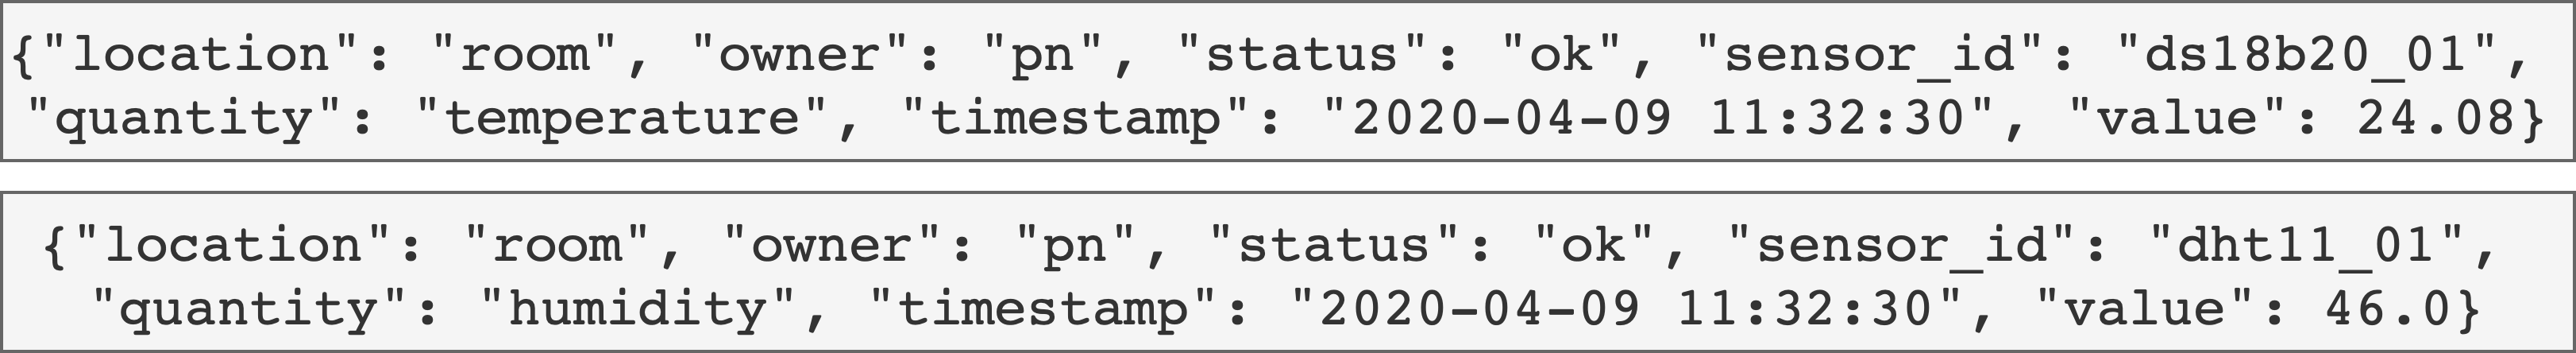
\includegraphics[width=1 \textwidth]{mqtt_message.png}
  \caption{Příklad dvou zpráv ve formátu JSON}
  \label{fig:mqtt_message}
\end{figure}

\subsection{Hierarchie zpráv} \label{subsec:message_hierarchy}
Při přenosu dat dochází k datovému toku ve směru od senzorů na broker. Broker pouze přijímá všechny zprávy, ale sám neposílá žádná data senzorům. Kvůli přehlednosti a jednotné struktuře posílaných zpráv je definována jasná hierarchie zpráv. Zprávy jsou odesílány do \textit{topiců}. Topic určuje téma dané zprávy a slouží k oddělení zpráv podle toho, od kterého odesílatele pocházejí a podle toho, kterou měřenou veličinu popisují. Každá zpráva je přiřazena právě jednomu tématu a název tohoto tématu určuje sám odesílatel zprávy. Příjemce zprávy pak jen musí znát název tématu, do kterého odesílatel publikuje zprávy. Témata jsou řetězce v kódování UTF-8 oddělená lomítky a jejich hierarchie není samotným protokolem nijak určená. Při návrhu hierarchie témat v projektu senzorického řešení domácnosti byl kladen důraz na univerzálnost a přirozenost s možností snadného rozšíření v budoucnu. \par
Základem všech názvů témat je slovo \textit{smarthome}. Za tímto slovem se přidá umístění senzoru a název měřené veličiny. Po spojení těchto třech slov vzniká název konkrétního topicu, kam senzor odesílá zprávy. V \cref{tab:mqtt_topic_structure} je uveden výčet všech topiců používaných v této práci.

\begin{table}[h]
\centering
 \begin{tabular}{|p{5.5cm}|} 
 \hline
  smarthome/location/quantity  \\
 \hline\hline
 smarthome/room/temperature \\ 
 smarthome/outside/temperature \\
 smarthome/room/humidity \\
 smarthome/room/illuminance \\
 smarthome/room/pressure \\
 smarthome/room/motion \\
 smarthome/room/door\_open \\
 smarthome/room/window\_open \\
 \hline
 \end{tabular}
 \caption{Výčet všech topiců, do kterých jsou odesílány zprávy}
 \label{tab:mqtt_topic_structure}
\end{table}

Hierarchie témat byla navržena tak, aby každá měřená fyzikální veličina měla svůj topic v závislosti na umístění. Díky této volbě je možné strukturu témat snadno rozšířit jak z hlediska lokalit (přidání dalších pokojů v chytré domácnosti - \textit{livingroom}, \textit{bedroom}, atd.), tak z hlediska veličin (například \textit{smoke\_detection}). Tento model hierarchie topiců také umožňuje spojovat témata do souvisejících celků. K těmto účelům slouží znaky + a \#. Symbol + nahrazuje jednu úroveň v topicu, například pro odebírání všech teplot nezávisle na lokaci nebo čidlu lze použít příkaz \textit{smarthome/+/temperature}. Symbol  \# nazuje slovo za posledním lomítkem, například pro odebírání všech veličin, které jsou měřeny v místnosti je možné použít příkaz \textit{smarthome/room/\#}. 

\section{Ukládání dat do databáze} \label{sec:database}

Databázový server odebírá nejvíce nadřazení topic \textit{smarthome/\#}, který zahrnuje všechny témata vypsané v \cref{tab:mqtt_topic_structure}.

Základní princip databáze, proč jsme se rozhodli pro použití databáze,  ... \\
Co je MongoDB (určení, využití, funkčnost, ... ) \\
Ukládání hodnot měřených veličin do MongoDB \\

\section{Webserver} \label{sec:webserver}

Popis backendu engine.py
Backend - z hlediska programování - jeden soubor engine.py, který zajišťuje serverování webové stránky, ukládání dat do databáze, sensor check, ... \\


